This appendix shows the postfit results of cross validated $\pod$-only
fit discussed in \prettyref{chap:Discussion}. The cross validation
error \eqref{eq:Vcosdelta} was minimized with a regularization strength
of $\lambda=1.4$. That is to say the penalty term in the test statistic
went from 
\[
\chi_{\text{Penalty}}^{2}=\left(\Delta\vec{y}\right)^{T}V^{-1}\left(\Delta\vec{y}\right)
\]
 to

\[
\chi_{\text{Penalty}}^{2}=\lambda\left(\Delta\vec{y}\right)^{T}V^{-1}\left(\Delta\vec{y}\right).
\]
We generally see the flux parameters have a slightly larger bias,
but reduced uncertainty. The cross section parameters are largely
unchanged. The first eight figures are the ND280 flux parameters.
The following eight are the unoscillated Super-Kamiokande (SK) flux
parameters. The next five are the cross section parameters. The final
two are the bin normalization parameters.

\includepdf[nup=2x4,pages={11-26,6-10},pagecommand=\thispagestyle{plain},width=2.9in]{Chapters/Figures/Discussion/P0DRegularizedvsTN324}

\includepdf[nup=2x4,pages={5-6},pagecommand=\thispagestyle{plain},width=2.9in]{Chapters/Figures/Discussion/Make2018PostFitFileAllParams_MultiTrackP0D_P0DOnly_Fit_v3r32_DataFit_WithSand_lambdaEq1\lyxdot 4_Sept15submit}
